\begin{savequote}[75mm]
It's going to take a lot of love to make things work out right.
\qauthor{Neil Young}
\end{savequote}

\chapter{Background Estimation in $VH$, $H\rightarrow \tau\tau$ Analysis}

\newthought{Despite the targeted event selection requirements defined in Chapter 6 it is not possible to eliminate all contributions from non- $VH,H\rightarrow\tau\tau$ events in the final di-tau mass spectrum.} Events originating from a different process that results in identical final state particles with sufficiently similar kinematics may also pass the analysis channel selections. Additionally, the reconstruction and identification algorithms defined in Chapter 3 are not 100\% accurate or efficient; it is possible that objects are mis-identified and events that do not truthfully contain all required final state particles mistakenly pass the analysis channel selections.\\

Correctly modeling these effects, collectively referred to as analysis backgrounds, is crucial to ensure accurate analysis results and to limit uncertainty of the final measurement. Several techniques are utilized in ATLAS analyses to model background contributions including fake factors (Section \ref{sec:ff_method}), shape studies, and embedding methods \cite{datadriven_bkg}.\\

Generally, data-driven methods for background estimation are preferred over MC-based methods. This is true for a variety of reasons including known mis-modeling effects in the current ATLAS simulation chain and the computing resources necessary to generate sufficient statistics to model specific background processes (see Chapter 3). Although incorporating production filters in the event generation stage can reduce the computing load in some cases they cannot be used for jet-based backgrounds like those that make up the majority of backgrounds in the $VH,H\rightarrow\tau\tau$ analysis. This is because the pile-up profile (which adds many jets to the event) is applied at a later simulation stage.\\

%% SEC: BACKGROUND TYPES
\section{Background Types}
There are two types of backgrounds for this analysis: events in which all 3 or 4 final state leptons are actually produced by some non $VH,H\rightarrow\tau\tau$ process and events in which some of the leptons are actually misidentified jets. These are referred to as irreducible backgrounds and fake backgrounds respectively. An MC-based method is used to estimate the irreducible background while a data-driven method is used model the fake backgrounds. A depiction of each method is shown in Figure \ref{fig:bkg_diag} where $\epsilon$ is the rate at which true, prompt objects pass the object criteria defined in Chapter 6 and $f$ is the object specific fake-factor as defined in Section \ref{sec:ff_method}. The two methods are described in further detail in the following sections.

\begin{figure}[htb!]
    \centering
    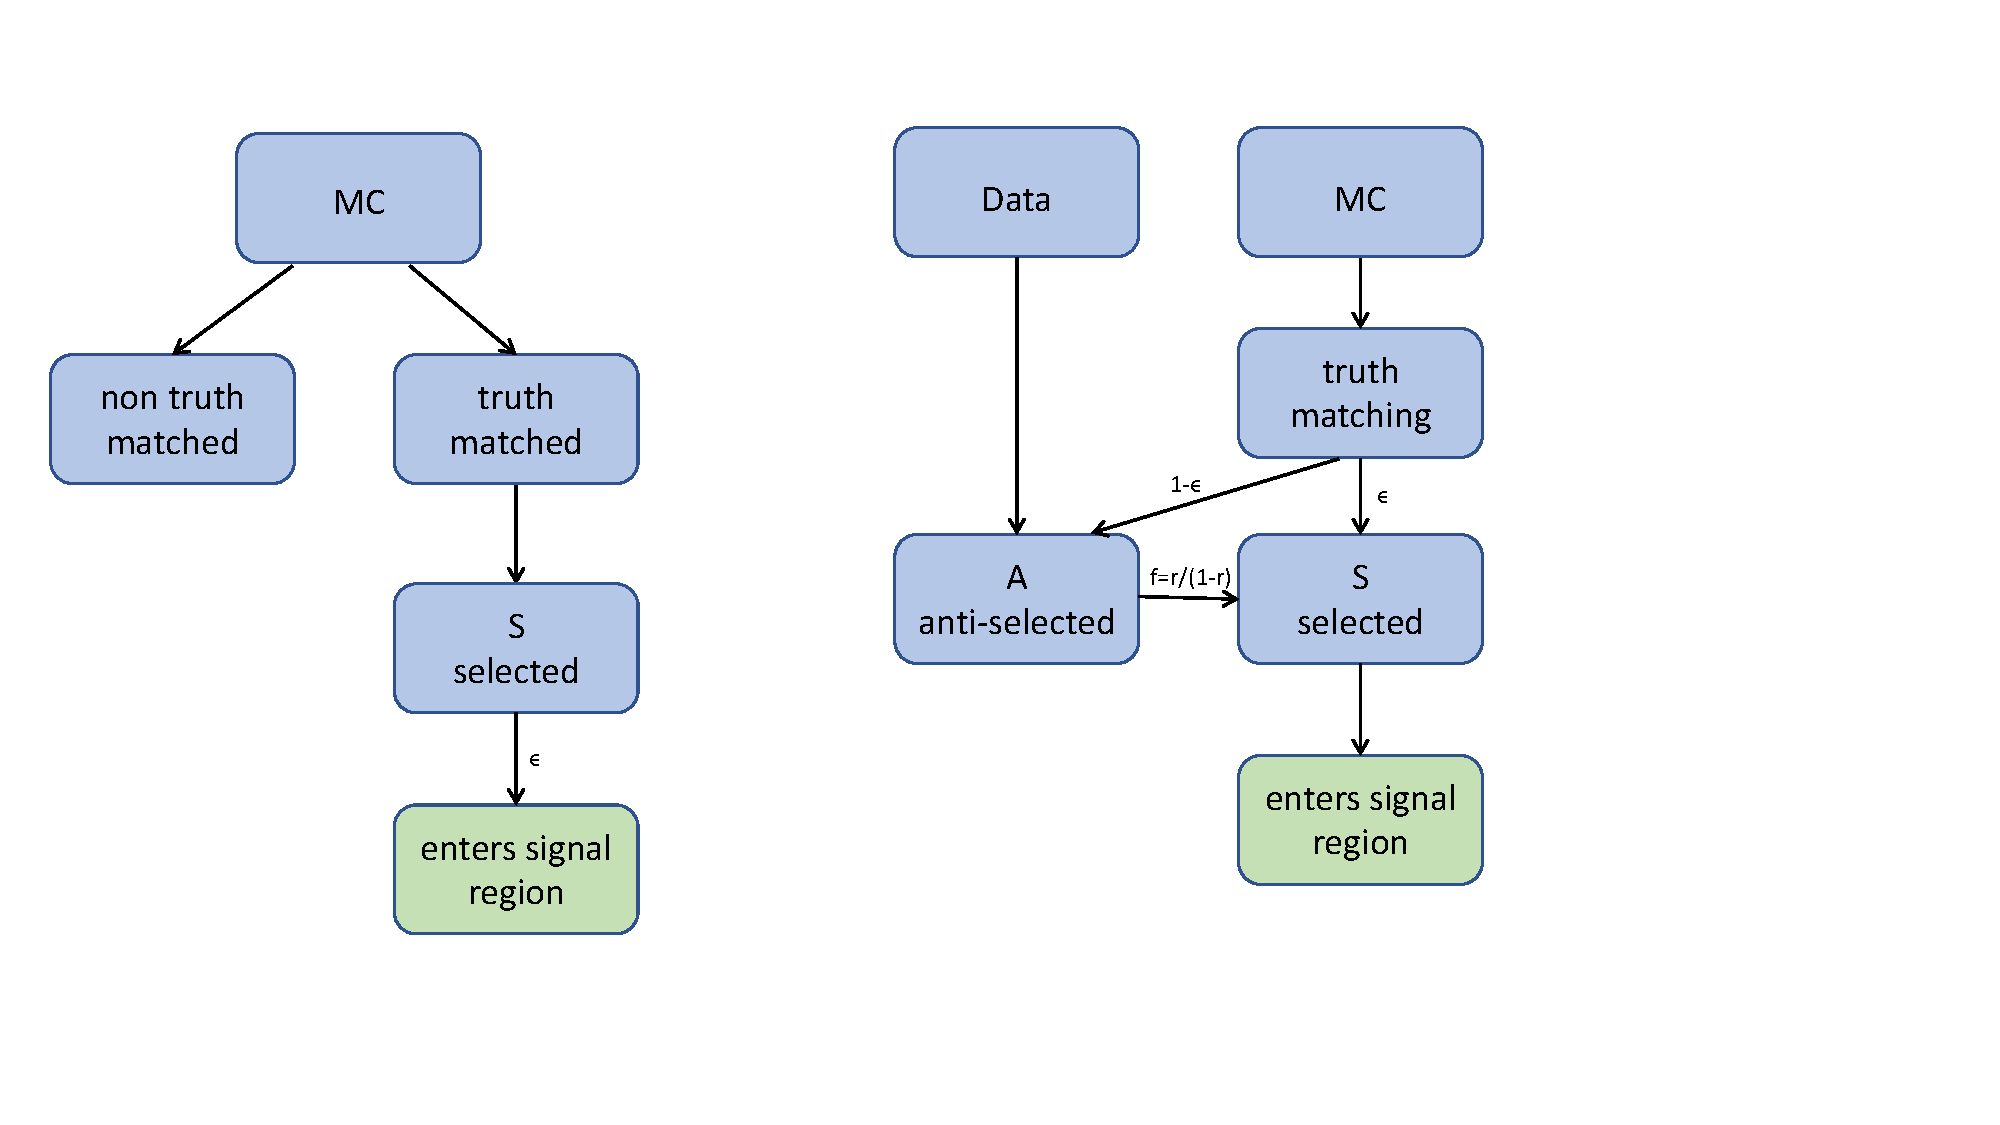
\includegraphics[width=5in]{figures/chapter7/background_diagram.pdf}
    \caption{Computing flow diagram for the MC-based irreducible background estimation (left) and data-driven fake background estimation (right).}
    \label{fig:bkg_diag}
\end{figure}
%% subsec: irreducible
\subsection{Irreducible Backgrounds}
Irreducible backgrounds containing true, prompt electrons, muons, and taus come mainly from non-resonant diboson events. These backgrounds are determined entirely from MC. The analysis category selections described in Chapter 6 are applied to MC samples of these processes. Objects in events which pass the category selection are then truth matched to ensure they originate from vector boson and Higgs decays. Events that pass truth matching are used to populate the irreducible background distributions. 

%% subsec: fakes
\subsection{Fake Backgrounds}
Events with fake objects are the primary source of background in all four analysis channels. These backgrounds are more difficult to estimate and are determined using the data-driven fake factor (FF) method which is the focus of the remainder of this chapter. The most common faked object in this analysis is the hadronic tau, and in Run-1 the tau FF method was sufficient for background modeling in three of the four analysis channels. The electron FF was used only in the WH lep-had channel and the muon FF method was not used in the final analysis \cite{vh_run1_paper}. For Run-2 the FF method is being studied for all three object types and the closure tests introduced in Section \ref{sec:closure} will aid in determining which methods to include in the final analysis. If it is found that one or two of the FF methods is sufficient to account for fake background contributions, the remaining methods will not be included to limit uncertainty on the final measurement. 

%% SEC: FAKE BACKGROUND METHOD
\section{The Fake Factor Method}\label{sec:ff_method}
Due to the relatively high number of final state objects (3 or 4 depending on the analysis category) and the potential for an event to include three different types of fake objects, modeling the fake background is one of the most challenging aspects of this analysis. The FF method was  developed in Run-1 for this purpose. It is a data-driven extrapolation method in which events with fake objects taken from a kinematically similar region (the fake region) are used to calculate a scale factor (the fake factor) which is applied to the final signal distribution to estimate the number of fake events. The mathematical derivation of this method is detailed in Section \ref{sec:derivation}, the FF measurements for each object type are described in Section \ref{sec:measurements}, and method validation studies are introduced in Section \ref{sec:closure}.

%%subsec: derivation
\subsection{Method Derivation}\label{sec:derivation}
The full mathematical description of the FF method is built on a set of object descriptors related to the different phases of the calculation. These terms are summarized in Table \ref{tab:ff_defs}. There are up to three identifiable final state objects in the WH channels and four in the ZH channels, thus it is necessary for the FF method to be able to acount for up to four faked objects. To illustrate the method construction the full derivation for the case in which only two final state objects can be faked (two object case) is presented in Section \ref{sec:2_obj} and the final equations for the three and four object cases are presented in Section \ref{sec:34_obj}.

\begin{table}[htb!]
    \centering
    \begin{tabular}{|c|c|p{4in}|}
    \hline
    \textbf{Term} & \textbf{Label} & \textbf{Definition} \\
    \hline
    \multicolumn{3}{|c|}{\textbf{Event Types}}\\
    \hline
    True Objects  & T & `real' objects: this is truth-level information that is unknown in data but is useful for method derivation \\
    Fake Objects  & F & inverse of true objects \\
    \hline
    \multicolumn{3}{|c|}{\textbf{Reconstructions}}\\
    \hline
    Selected & S & Object passes selection criteria (Chapter 6)\\
    Anit-selected & A & Object passes fake criteria (Section \ref{sec:measurements})\\
    \hline
    \multicolumn{3}{|c|}{\textbf{Rates}}\\
    \hline
    Fake rate & r & Rate at which Fake Objects (F) are reconstructed as selected (S)\\
    Real efficiency & $\epsilon$ & Rate at which True Objects (T) are reconstructed as selected (S)\\
    Fake Factor & f & $\frac{r}{1-r}$ \\
    \hline
    \end{tabular}
    \caption{Fake factor method definitions.}
    \label{tab:ff_defs}
\end{table}

\subsubsection{Two Object Case}\label{sec:2_obj}
The ultimate goal of the FF method is to calculate the number of events of a certain type (ie $N_{FF}$ for number of events where both of the final state objects are actually fakes) that enter the signal region. However, this is truth-level information which is inherently unknowable in data. Thus, the FF method is used to compute these numbers in terms of quantities that are measurable in data.\\

First, consider event types that can enter the signal region through the FF method. These events must have at most one true object (if they had two true objects they would enter the signal region through normal selection). They can also include any number of fake objects but only a total of two objects can ultimately pass the object identification criteria (be selected). In this derivation it is assumed that true objects are always selected; as discussed in Chapter 3 this is not strictly true and a correction to account for this assumption is described in Section \ref{sec:mc_corr}. The probability that a fake object is selected is $r$ and the probability it is not selected (anti-selected) is $1-r$. The process for measuring $r$ is described in Section \ref{sec:measurements}. A summary of event types and their corresponding probabilities for entering the signal region is shown in Table \ref{tab:ff_1}. The fake rate for an object depends on its kinematics and so object ordering is necessary.\\

\begin{table}[htb!]
    \centering
    \begin{tabular}{|c|c|}
    \hline
        \textbf{Event Type} &  \textbf{Probability of Entering Signal Region}\\
        \hline
        $\text{TF}_1$ & $r$\\
        $\text{F}_1\text{F}_2$ & $r_1 r_2$\\
        $\text{TF}_1\text{F}_2$ & $(r_1 (1-r_2))+(r_2 (1-r_1))$\\
        $\text{F}_1\text{F}_2\text{F}_3$ & $(r_1 r_2(1-r_3))+(r_1 r_3(1-r_2))+(r_2r_3(1-r_1))$\\
        $\vdots$ & $\vdots$\\
        \hline
    \end{tabular}
    \caption{Truth-level event types and their probabilities of entering the Signal Region.}
    \label{tab:ff_1}
\end{table}

It is clear from Table \ref{tab:ff_1} that the complexity of the selection probabilities rapidly increases with the number of fake objects considered in the event due to the multiple allowed selection combinations. As shown in Section \ref{sec:measurements}, in this analysis the fake rates for all object types are less than one. Thus, as the number of fake rates considered increases, the probability of a specific individual reconstruction decreases.  Therefore, the remainder of this derivation will consider only first-order events (events with two objects). In the Run-1 analysis this approximation was sufficient for background modeling in all four signal channels and initial studies (Section \ref{sec:closure}) indicate this is also sufficient for the Run-2 analysis.\\

Now the event types can be written in terms of data-set qualities: whether the objects are reconstructed as selected or anti-selected. The three possible first-order two object cases and their reconstructions are shown in Table \ref{tab:ff_2}. The number of events with each of these reconstructions are shown in Table \ref{tab:ff_3}.\\

\pagebreak

\begin{table}[htb!]
    \centering
    \begin{tabular}{|c|c|}
    \hline
        \textbf{Event Type} & \textbf{Reconstructions} \\
        \hline
        $\text{F}_1\text{T}$ & SS, AS\\
        $\text{TF}_2$ & SS, SA\\
        $\text{F}_1\text{F}_2$ & SS, SA, AS, AA\\
        \hline
    \end{tabular}
    \caption{Possible reconstructions for truth event types.}
    \label{tab:ff_2}
\end{table}

\begin{table}[htb!]
    \centering
    \begin{tabular}{|c|c|c|}
    \hline
    \textbf{Event Type} & \textbf{Reconstruction} & \textbf{Number of Events}\\
    \hline
       \multirow{2}{*}{$\text{F}_1\text{T}$} & SS & $r_1 \times N_{F_1T}$\\
        & AS & $(1-r_1)\times N_{F_1T}$\\
        \hline
        \multirow{2}{*}{$\text{TF}_2$} & SS & $r_2\times N_{TF_2}$\\
        & SA & $(1-r_2)\times N_{TF_2}$\\
        \hline
        \multirow{4}{*}{$\text{F}_1\text{F}_2$} & SS & $r_1 r_2 \times N_{F_1F_2}$\\
        & SA & $r_1(1-r_2)\times N_{F_1F_2}$\\
        & AS & $(1-r_1)r_2\times N_{F_1F_2}$\\
        & AA & $(1-r_1)(1-r_2)\times N_{F_1F_2}$\\
        \hline
    \end{tabular}
    \caption{The number of events that are reconstructed a certain way.}
    \label{tab:ff_3}
\end{table}

Now the total number of each reconstruction can be found by summing across the underlying event types.
\begin{gather*}
    N_{SS}=(r_1 N_{F_1T})+(r_2 N_{TF_2}) + (r_1r_2 N_{F_1F_2})\\
    N_{SA}=((1-r_2) N_{TF_2})+(r_1(1-r_2) N_{F_1F_2})\\
    N_{AS}=((1-r_1)\times N_{F_1T})+((1-r_1)r_2 N_{F_1F_2})\\
    N_{AA}=(1-r_1)(1-r_2) N_{F_1F_2}
\end{gather*}
\noindent Ultimately, only reconstructions with two selected objects (SS reconstructions) will pass the signal region selections. It is thus necessary to express $N_{SS}$ in terms of the other measurable quantities $N_{SA}$, $N_{AS}$, and $N_{AA}$.\\

Begin by inverting the equation for $N_{AA}$:
\begin{equation}\label{eq:1}
N_{F_1F_2}=\frac{N_{AA}}{(1-r_1)(1-r_2)}  
\end{equation}

\noindent Now consider the equation for $N_{AS}$:
\begin{flalign}
& N_{AS}=((1-r_1) N_{F_1T})+((1-r_1)r_2 N_{F_1F_2}) \rightarrow \nonumber\\
& (1-r_1)N_{F_1T}=N_{AS}-(1-r_r)r_2N_{F_1F_2} \rightarrow \nonumber\\ 
& N_{F_1T}=\frac{N_AS}{(1-r_1)}-r_2N_{F_1F_2}\label{eq:2}
\end{flalign}
\noindent Substitute equation \ref{eq:1} into equation \ref{eq:2}:
\begin{equation*}
    N_{F_1T}=\frac{N_{AS}}{1-r_1}-\frac{r_2 N_{AA}}{(1-r_1)(1-r_2)}
\end{equation*}
\noindent Define the fake factor $f$ of an object as $f=r/(1-r)$ and finally
\begin{equation}\label{eq:3}
    N_{F_1T}=\frac{N_{AS}}{1-r_1}-\frac{f_2N_{AA}}{1-r_1}.
\end{equation}
\noindent Repeating the same procedure for $N_{SA}$ gives:
\begin{equation}\label{eq:4}
    N_{TF_2}=\frac{N_{SA}}{1-r_2}-\frac{f_1N_{AA}}{1-r_2}.
\end{equation}

Finally, $N_{SS}$ can be written in terms of equations \ref{eq:2} - \ref{eq:4}.
\begin{flalign}
& N_{SS}=r_1N_{F_1T} + r_2 N_{TF_2} + r_1r_2 N_{F_1F_2}\rightarrow \nonumber \\
& N_{SS}=r_1\Big[\frac{N_{AS}}{1-r_1}-\frac{f_2N_{AA}}{1-r_1}\Big]+r_2\Big[\frac{N_{SA}}{1-r_2}-\frac{f_1N_{AA}}{1-r_2}\Big] \nonumber\\
& N_{SS}=f_1[N_{AS}-f_2N_{AA}]+f_2[N_{SA}-f_1N_{AA}]+f_1f_2N_{AA} \nonumber\\
& N_{SS}=f_1N_{AS}+f_2N_{SA}-f_1f_2N_{AA}
\end{flalign}
\noindent Using the object specific fake factors it is possible to calculate the number of events with fake objects that enter the signal region in terms of individual event reconstructions.

\subsubsection{Three and Four Object Cases}\label{sec:34_obj}
The derivations for the three and four object cases proceed similarly and result in:
\begin{multline*}
    N_{SSS}=f_3N_{SSA}-f_2f_3N_{SAA}+f_1f_2f_3N{AAA}-f_1f_3N_{ASA}\\
    +f_2N_{SAS}-f_1f_2N{AAS}+f_2N_{ASS}
\end{multline*}
\noindent for the three object case and 
\begin{multline*}
    N_{SSSS}=f_1N{ASSS}+f_2N_{SASS}+f_3N_{SSAS}+f_4N_{SSSA}-f_1f_4N_{ASSA}-f_2f_4N_{SASA}\\
    -f_3f_4N_{SSAA}-f_2f_3N_{SAAS}-f_1f_2N_{AASS}-f_1f_3N_{ASAS}+f_1f_2f_4N_{AASA}\\
    +f_1f_3f_4N_{ASAA}+f_2f_3f_4N_{SAAA}+f_1f_2f_3N_{AAAS}-f_1f_2f_3f_4N_{AAAA}
\end{multline*}
\noindent for the four object case.

%% SEC: FF MEASUREMENTS
\section{Fake Factor Measurements}\label{sec:measurements}
The fake rate is measured in a phase-space region that is enriched in fake object and should contain minimal true objects (referred to as the Fake Region). When measured in such a region the fake rate, $r$ is defined as $r=\frac{N_S}{N_S+N_A}$. The fake factor is then $f=\frac{r}{1-r}=\frac{N_S}{N_A}$. The fake rates are sensitive to the underlying physics of the event and so in order to model the fake backgrounds accurately it is necessary to select a Fake Region that is as kinematically similar to the Signal Region as possible. For this analysis, the Fake Region is the $Z/\gamma^*\rightarrow\mu\mu$ region which is further defined in Section \ref{sec:zmumu}. After constructing the Fake Region using data, the number of selected and anti-selected are measured and the fake rates and factors are calculated.\\

The fake rates and factors of each object are measured separately for the ZH and WH channels due to a number of differences in the kinematics of the categories. This includes the presence of additional MET in the WH channels and differing object origins between the two categories.

%% subsec: zmumu region
\subsection{Fake Region}\label{sec:zmumu}
The fake rates and factors for all three object types are measured in the $Z/\gamma^*\rightarrow\mu\mu+\text{jets}$ region (referred to as $Z\rightarrow\mu\mu$ for short). The muons that originate from the $Z$ decay should be the only true leptons in the event and thus any additional lepton is likely a mis-identified jet (fake).\\

The $Z\rightarrow\mu\mu$ region is constructed by first requiring at least one of the two muon triggers used in the signal region (\verb!HLT_2mu14! and \verb!HLT_mu26_ivarmedium!) is fired. Events are additionally required to have two isolated oppositely charged muons with a combined mass between 71 and 111 GeV and no b-jets. An example of the $Z\rightarrow\mu\mu$ purity in this region is shown in Figure \ref{fig:zmass_plots}: the vast majority of MC events that pass the Fake Region selection are $Z\rightarrow\mu\mu$ processes.

\begin{figure}[h]
    \begin{subfigure}
        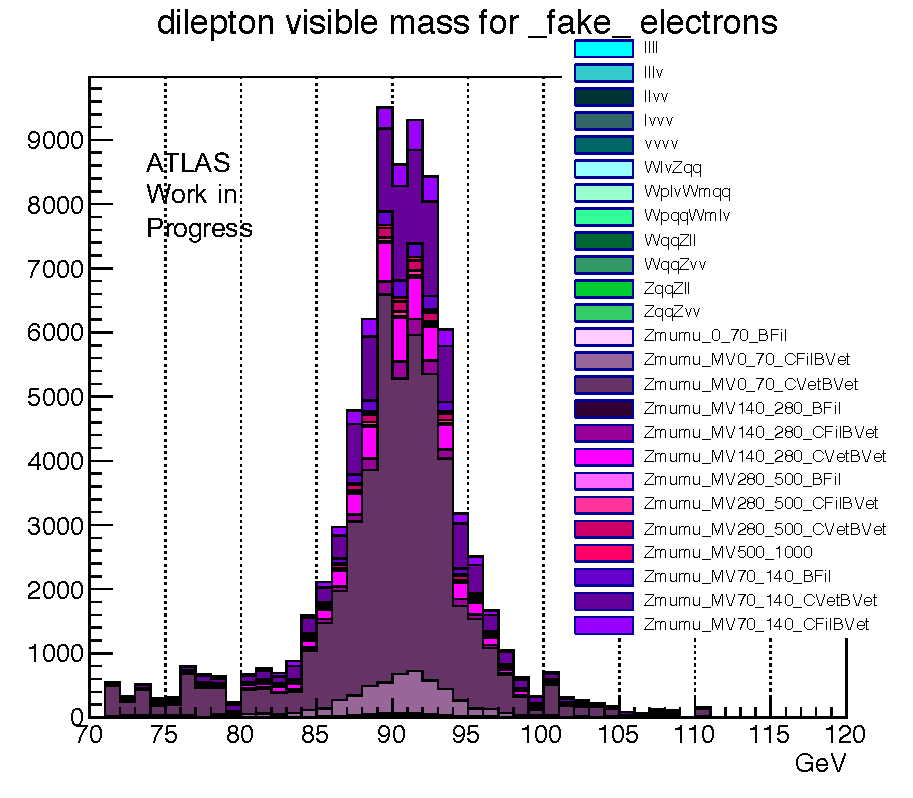
\includegraphics[width=2.8in]{figures/chapter7/zmass_fakes.pdf}
    \end{subfigure}
    \begin{subfigure}
        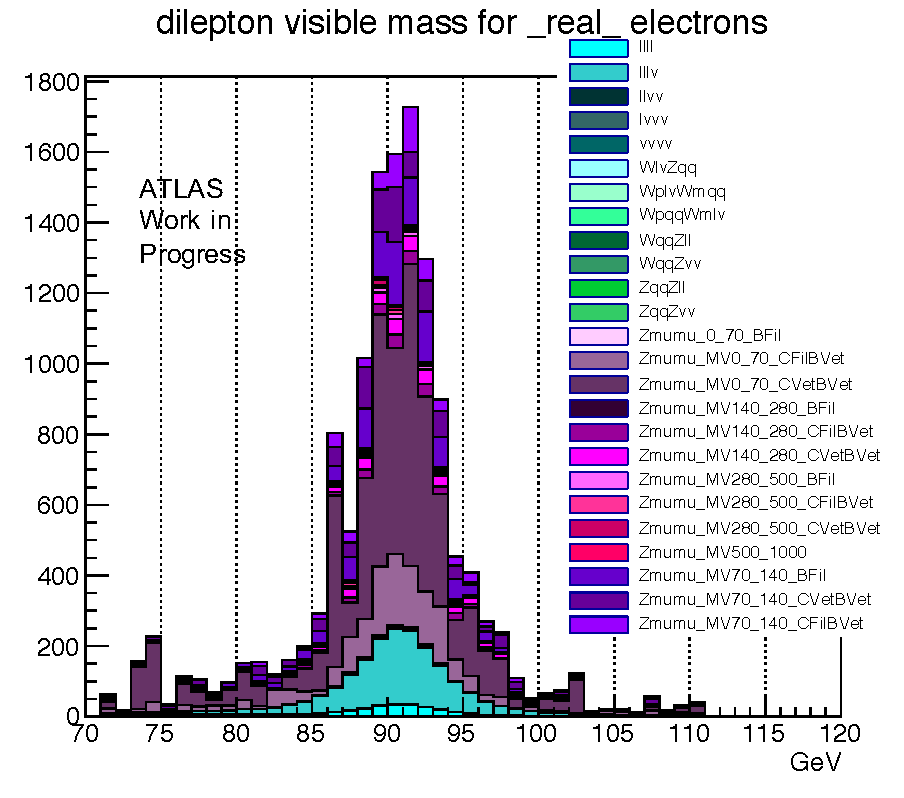
\includegraphics[width=2.8in]{figures/chapter7/zmass_reals.pdf}
    \end{subfigure}
    \caption{Di-muon visible mass in the $Z\rightarrow\mu\mu$ Fake Region for events with an anti-selected electron (left) and a selected electron (right).}
    \label{fig:zmass_plots}
\end{figure}

%% subsec: fake candidates
\subsection{Fake Candidate Selection}
Anti-selected objects are required to pass the same object criteria described in Chapter 6 with the following differences:
\begin{itemize}
    \item Anti-selected electrons must fail the Loose ID operating point rather than pass the Medium ID operating point.
    \item Anti-selected taus must fail rather than pass the BDT-Medium ID operating point but pass a loosened ID of 0.7$\times$BDT-Loose.
    \item Anti-selected muons must fail rather than pass the Gradient Isolation operating point.
\end{itemize}
\noindent The overlap removal resolution order for anti-selected objects is taus $>$ electrons $>$ muons. If two anti-selected objects of the same type overlap, the one with the greater $p_T$ is chosen.

%% subsec: fake electrons
\subsection{Fake Electrons}
Fake electrons can originate from a variety of sources including mis-identified jets, light meson decays, heavy flavor hadron decays, and photon conversions. The electron ID algorithm depends heavily on $p_T$ and $\eta$ and so the electron FRs and FFs are measured for a 2D phase-space of seven $\eta$ bins and four $p_T$ bins. The bin divisions were initially set in Run-1 to achieve roughly consistent statistical error across bins. This same binning is currently used for the Run-2 analysis with an additional low $p_T$ bin. The FRs and FFs are measured separately for the ZH and WH channels due to different fake electron compositions as described further in the following section. The ZH Fake Region applies a tighter di-muon mass cut of 81-101 GeV while the WH Fake Region loosens the mass cut to 61-121 GeV.\\

The electron FRs measured in the full 2017 data-set are shown in Figures \ref{fig:zh_frs} and \ref{fig:wh_frs} and summarized in Tables \ref{tab:zh_frs} and \ref{tab:wh_frs}. The highest $p_T$ bin has low statistics and has been removed from the plots for ease of presentation. The final analysis will use the full Run-2 data-set which will improve the statistics in this bin and yield a more reliable FR measurement.\\

\begin{table}[htb!]
    \centering
    \begin{tabular}{|c|c|c|c|c|}
    \hline
    $\eta$ & $5<p_T<10$ & $10<p_T<15$ & $15<p_T<20$ & $20<p_T$ \\
    \hline
    -2.5 - -2.01 & 0.090 & 0.039 & 0.072 & 0.455 \\
    -2.01 - -1.52 & 0.083 & 0.139 & 0.243 & 0.337 \\
    -1.37 - -0.46 & 0.104 & 0.152 & 0.263 & 0.321\\
    -0.46 - 0.46 & 0.179 & 0.279 & 0.275 & 0.297\\
    0.46 - 1.37 & 0.106 & 0.154 & 0.280 & 0.313\\
    1.52 - 2.01 & 0.093 & 0.129 & 0.257 & 0.295\\
    2.01 - 2.5 & 0.085 & 0.039 & 0.077 & 0.381\\
    \hline
    \end{tabular}
    \caption{Measured electron fake rate for the ZH channels.}
    \label{tab:zh_frs}
\end{table}

\begin{figure}[htb!]
    \centering
    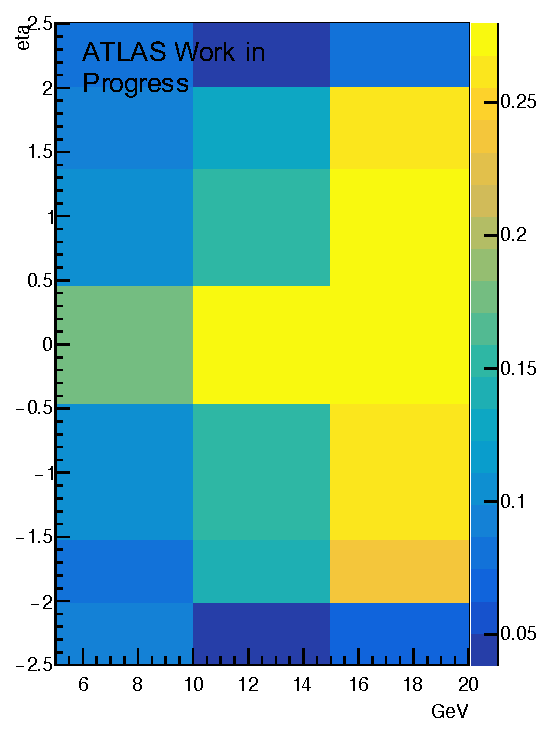
\includegraphics[width=3in]{figures/chapter7/data17_zh_frs.pdf}
    \caption{Measured electron fake rate for the ZH channels.}
    \label{fig:zh_frs}
\end{figure}

\begin{table}[htb!]
    \centering
    \begin{tabular}{|c|c|c|c|c|}
    \hline
    $\eta$ & $5<p_T<10$ & $10<p_T<15$ & $15<p_T<20$ & $20<p_T$ \\
    \hline
    -2.5 - -2.01 & 0.096 & 0.045 & 0.095 & 0.437 \\
    -2.01 - -1.52 & 0.086 & 0.155 & 0.245 & 0.330 \\
    -1.37 - -0.46 & 0.109 & 0.164 & 0.274 & 0.330\\
    -0.46 - 0.46 & 0.181 & 0.292 & 0.295 & 0.308\\
    0.46 - 1.37 & 0.109 & 0.171 & 0.307 & 0.310\\
    1.52 - 2.01 & 0.097 & 0.141 & 0.286 & 0.308\\
    2.01 - 2.5 & 0.092 & 0.045 & 0.099 & 0.374\\
    \hline
    \end{tabular}
    \caption{Measured electron fake rate for the WH channels.}
    \label{tab:wh_frs}
\end{table}

\begin{figure}[htb!]
    \centering
    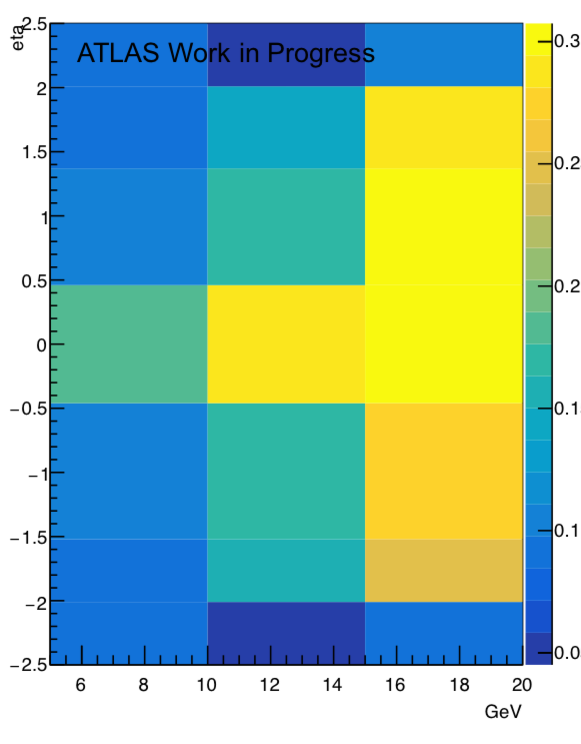
\includegraphics[width=3in]{figures/chapter7/data17_wh_frs.pdf}
    \caption{Measured electron fake rate for the WH channels.}
    \label{fig:wh_frs}
\end{figure}

The FRs increase with increasing $p_T$ and are highly symmetric in $\eta$ (thus the analysis could use only four bins of $|\eta|$ as is done for taus).

\pagebreak

\subsubsection{Type and Origin Studies}
In Run-1 it was found that the electron compositions varied significantly between the ZH and WH channels. In particular, the fake electrons in ZH channel were predominately mis-identified jets. The tighter di-muon mass requirement for the ZH FR measurement reduced the amount of final state radiation and thus the number of photon conversion fake electrons. On the other hand, fake electrons in the WH channel were equally split between mis-identified jets and converted photons. The low di-muon mass range (61-81 GeV) is enriched in $Z\rightarrow\mu\mu$ decays with additional final state radiation and thus loosened mass requirement for the WH FR measurement increased the number of photon conversion fake electrons.\\

Studies are on-going to understand if these same Fake Region definitions are necessary and sufficient for the Run-2 electron FR measurement. The electron composition of the ZH Fake Region is shown in Figure \ref{fig:zh_fr_origins} and the composition of the WH Fake Region is shown in Figure \ref{fig:wh_fr_origins}. The electron composition for the ZH and WH signal regions are shown in Figures xx and xx. These plots all use the E/Gamma Working Group supported electron origin classification scheme which is summarized in Table \ref{tab:elec_origin}.\\

\begin{table}[htb!]
    \centering
    \begin{tabular}{|c|c|}
    \hline
    \textbf{Number} & \textbf{Electron Origin}\\
    \hline
    0 & Not Defined\\
    \hline
    \multicolumn{2}{|c|}{\textbf{Prompt Objects}}\\
    \hline
    1 & Prompt Electron \\
    2 & Single Muon \\
    3 & Single Photon \\
    4 & Single Tau \\
    \hline
    \multicolumn{2}{|c|}{\textbf{Conversions}}\\
    \hline
    5 & Photon Conversion \\
    \hline
    \multicolumn{2}{|c|}{\textbf{Particle Decays}}\\
    \hline
    6 & Dalitz Decay\\
    8 & Muon Decay\\
    9 & Leptonic Tau Decay\\
    12 & W Decay\\
    13 & Z Decay\\
    14 & Higgs Decay \\
    28 & $J/\Psi$ Decay\\
    \hline
    \multicolumn{2}{|c|}{\textbf{Jets}}\\
    \hline
    10 & Top Jet\\
    11 & QCD Showering\\
    23 & Light Jet\\
    24 & Strange Jet\\
    25 & Charm Jet\\
    26 & Bottom Jet\\
    27 & $c\bar{c}$ Production\\
    \hline
    \end{tabular}
    \caption{Electron origin numbering scheme.}
    \label{tab:elec_origin}
\end{table}

\begin{figure}[htb!]
    \begin{subfigure}
        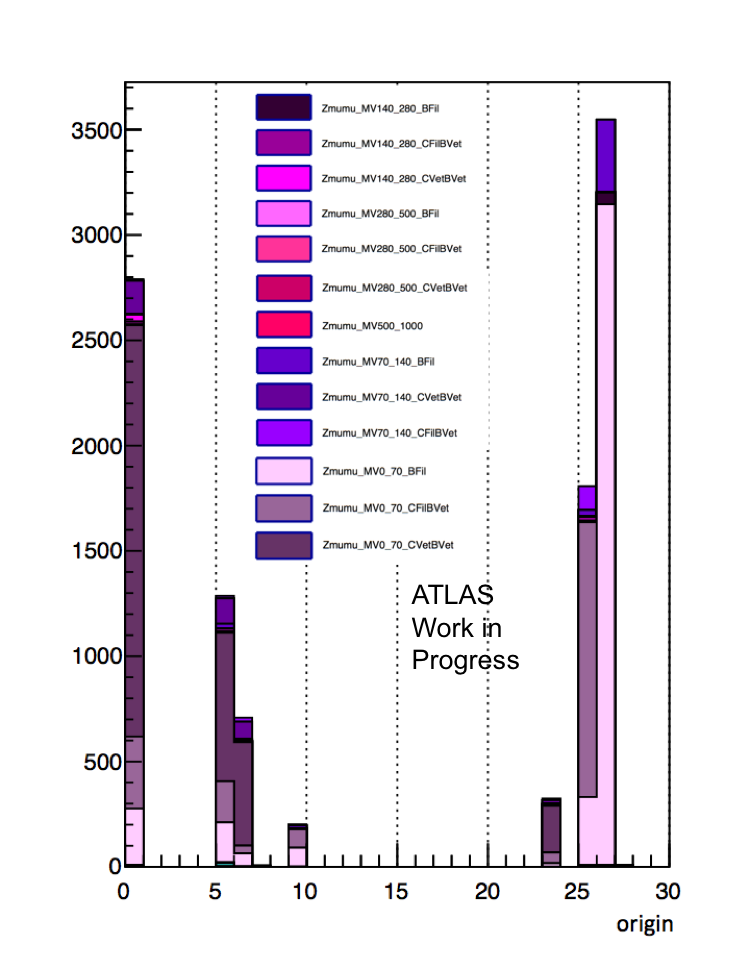
\includegraphics[width=2.8in,height=3.2in]{figures/chapter7/selected_zh_fr.png}
    \end{subfigure}
    \begin{subfigure}
        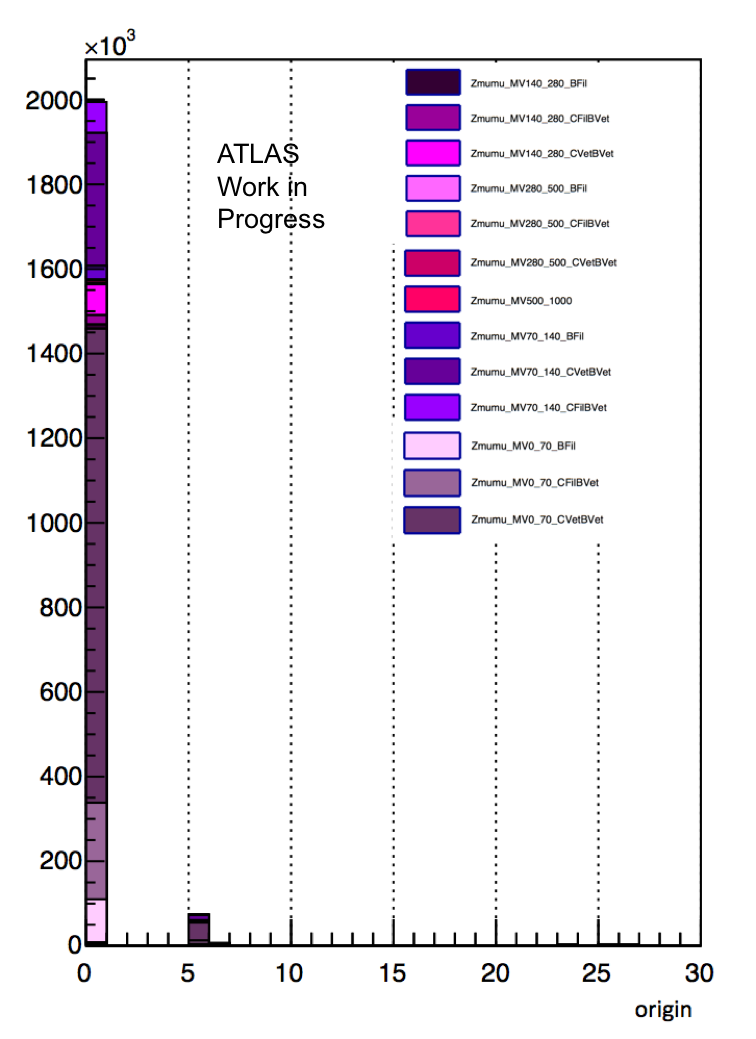
\includegraphics[width=2.5in,height=3.1in]{figures/chapter7/zh_anti_fr.png}
    \end{subfigure}
    \caption{Electron origins (as defined in Table \ref{tab:elec_origin} in the ZH Fake Region. Selected electrons on the left and anti-selected electrons on the right.}
    \label{fig:zh_fr_origins}
\end{figure}

\pagebreak

\begin{figure}[htb!]
    \begin{subfigure}
        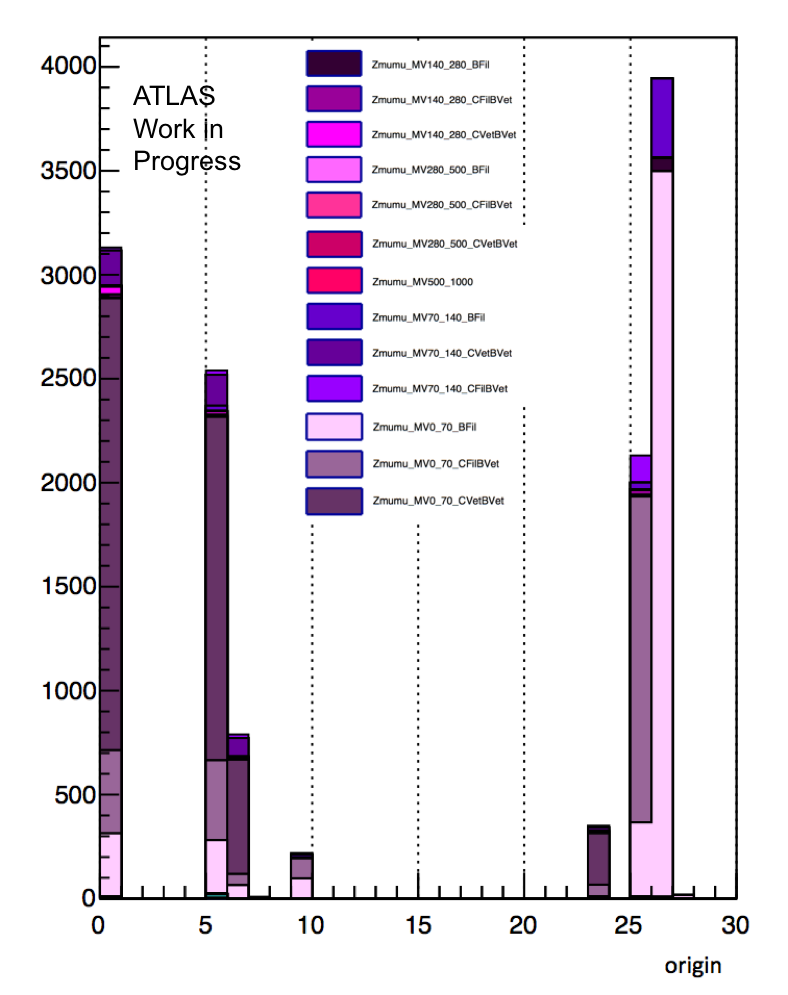
\includegraphics[width=2.8in]{figures/chapter7/selected_wh_fr.png}
    \end{subfigure}
    \begin{subfigure}
        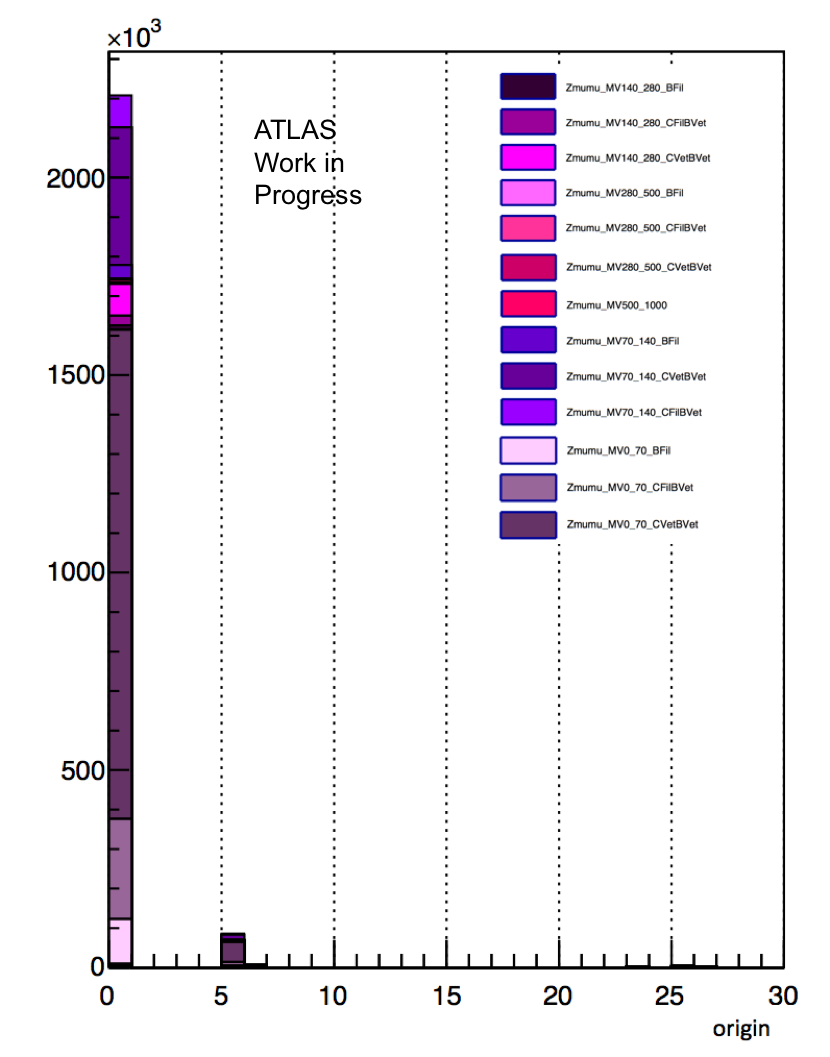
\includegraphics[width=2.8in]{figures/chapter7/wh_anti_fr.png}
    \end{subfigure}
    \caption{Electron origins in the WH Fake Region. Selected electrons on the left and anti-selected electrons on the right.}
    \label{fig:wh_fr_origins}
\end{figure}

**FILL IN ANALYSIS OF PLOTS.**

\pagebreak

%% subsec: taus and muons
\subsection{Fake Taus and Muons}
\subsubsection{Fake Taus}
The tau FRs and FFs are measured in a 2D phase-space of 5 $p_T$ bins and 3 $|\eta|$ bins. The FFs and FRs are measured separately for the ZH and WH categories. In the fake tau measurement these categories are separated by requiring MET$>$20 GeV for the WH measurement; there is no MET requirement for the ZH measurement. The FRs and FFs for 1-prong taus are typically higher than those of 3-prong taus and so they are measured separately for these categories as well. The tau FRs measured in the full 2017 data-set are summarized in Tables \ref{tab:zh_1p_tau_frs} - \ref{tab:wh_3p_tau_frs}.\\

\begin{table}[htb!]
    \centering
    \begin{tabular}{|c|c|c|c|}
    \hline
    $p_T$ (GeV) & $|\eta|<0.8$ & $0.8<|\eta|<1.37$ & $1.37<|\eta|<2.5$\\
    \hline
    $25<p_T<30$ & 0.168 & 0.146 & 0.158\\
    $30<p_T<35$ & 0.161 & 0.151 & 0.149\\
    $35<p_T<40$ & 0.157 & 0.149 & 0.140\\
    $40<p_T<60$ & 0.131 & 0.114 & 0.118\\
    $60<p_T$ & 0.093 & 0.083 & 0.079\\
    \hline
    \end{tabular}
    \caption{Measured 1-prong tau fake rates for the ZH channels.}
    \label{tab:zh_1p_tau_frs}
\end{table}

\begin{table}[htb!]
    \centering
    \begin{tabular}{|c|c|c|c|}
    \hline
    $p_T$ (GeV) & $|\eta|<0.8$ & $0.8<|\eta|<1.37$ & $1.37<|\eta|<2.5$\\
    \hline
    $25<p_T<30$ & 0.032 & 0.034 & 0.033\\
    $30<p_T<35$ & 0.031 & 0.031 & 0.033\\
    $35<p_T<40$ & 0.030 & 0.031 & 0.030\\
    $40<p_T<60$ & 0.025 & 0.023 & 0.021\\
    $60<p_T$ & 0.016 & 0.011 & 0.001\\
    \hline
    \end{tabular}
    \caption{Measured 3-prong tau fake rates for the ZH channels.}
    \label{tab:zh_3p_tau_frs}
\end{table}

\begin{table}[htb!]
    \centering
    \begin{tabular}{|c|c|c|c|}
    \hline
    $p_T$ (GeV) & $|\eta|<0.8$ & $0.8<|\eta|<1.37$ & $1.37<|\eta|<2.5$\\
    \hline
    $25<p_T<30$ & 0.133 & 0.102 & 0.132\\
    $30<p_T<35$ & 0.125 & 0.109 & 0.121\\
    $35<p_T<40$ & 0.117 & 0.113 & 0.112\\
    $40<p_T<60$ & 0.106 & 0.091 & 0.098\\
    $60<p_T$ & 0.083 & 0.069 & 0.068\\
    \hline
    \end{tabular}
    \caption{Measured 1-prong tau fake rates for the WH channels.}
    \label{tab:wh_1p_tau_frs}
\end{table}

\begin{table}[htb!]
    \centering
    \begin{tabular}{|c|c|c|c|}
    \hline
    $p_T$ (GeV) & $|\eta|<0.8$ & $0.8<|\eta|<1.37$ & $1.37<|\eta|<2.5$\\
    \hline
    $25<p_T<30$ & 0.029 & 0.026 & 0.027\\
    $30<p_T<35$ & 0.027 & 0.025 & 0.025\\
    $35<p_T<40$ & 0.024 & 0.022 & 0.024\\
    $40<p_T<60$ & 0.019 & 0.022 & 0.021\\
    $60<p_T$ & 0.014 & 0.012 & 0.013\\
    \hline
    \end{tabular}
    \caption{Measured 3-prong tau fake rates for the WH channels.}
    \label{tab:wh_3p_tau_frs}
\end{table}

\pagebreak

Jets can be formed through quark-initiated and gluon-initiated processes and the probability for a hadronic jet to be mis-identified as a tau depends on its origin. Thus the central challenge of modeling the fake tau background in this analysis is ensuring that the jet origin composition in the Fake Region matches that of the Signal Region as closely as possible. Studies to ensure this for the Run-2 analysis are on-going.\\ 

\subsubsection{Fake Muons}
The muon FRs and FFs are measured in a 2D phase-space of 3 $p_T$ bins and 3 $\eta$ bins. Initial muon fake rates measured in a subset of 2017 data are shown in Table \ref{tab:muon_frs}.

\begin{table}[htb!]
    \centering
    \begin{tabular}{|c|c|c|c|}
    \hline
    $p_T$ (GeV) & $-2.5<\eta<-1.2$ & $-1.2<\eta<1.2$ & $1.2<\eta<2.5$\\
    \hline
    $p_T<15$ & 0.666 & 0.422 & 0.700\\
    $15<p_T<25$ & 0.631 & 0.440 & 0.691\\
    $25<p_T$ & 0.673 & 0.436 & 0.783\\
    \hline
    \end{tabular}
    \caption{Preliminary measured muon fake rates.}
    \label{tab:muon_frs}
\end{table}

There are multiple challenges involved in measuring the muon FRs. These include tuning the isolation requirement on the anti-selected muons to appropriately select jets faking muons but not muons produced inside jets and understanding the interaction of trigger-based and offline isolation requirements.

%%subsec: MC correction
\subsection{MC Corrections}\label{sec:mc_corr}
The FF method derivation described in Section \ref{sec:derivation} relies on the assumption that all true objects pass their corresponding selection requirements. It is additionally assumed that all objects passing selection requirements in the Fake Region are fakes. Neither assumption is strictly true but they can both be easily accounted for in the final measurement.\\

To account for these assumptions, the fake factor (previously $f(p_T,\eta)=\frac{N_S}{N_A}$ is redefined as:
\begin{equation*}
    f(p_T,\eta)=\frac{N_S^{data}-N_S^{MC}}{N_A^{data}-N_A^{MC}}.
\end{equation*}
\noindent The MC terms are measured by combining truth-matched prompt objects from all physics processes that could pass the signal region selections (Chapter 6). In practice these are primarily di-boson processes. The MC-based subtraction is included in the numerator to remove contamination of true objects in the Fake Region and in the denominator to account for true objects that do not pass the object selection criteria.\\

These corrections are not included in the initial FR measurements presented above but will be incorporated in the final background model.

%% SEC: FF SOFTWARE
\section{Fake Factor Software}
In order to measure the fake background contributions to the final analysis it is necessary to apply the measured FFs to the data in each analysis channel according to the equations derived in Section \ref{sec:derivation}. In practice, this requires a complex software implementation. The FF software must first incorporate modified analysis channel selections that do not impose object identification requirements (or isolation requirements in the muon case). It must then construct all possible allowed combinations of final state objects for each data event and save each combination as a new event that is weighted appropriately according to the FF equations. These weighted events then populate the background model in each analysis category.\\

For the $VH,H\rightarrow\tau\tau$ analysis in particular, in order to accommodate all the studies necessary to validate the FF background model, the FF software must be highly flexible. It must be possible to consider multiple combinations of fake object types (as few as one or as many as three),  different numbers of final state objects that are faked, and various numbers of fake candidates considered per event. Furthermore, the FF software must interface with the pre-selection and selection criteria for all four analysis channels as well as multiple orthogonal control regions that are used to validate the background model.\\

Other ATLAS analyses have implemented a data-based FF background model (see e.g. \cite{fake_tau_paper} and \cite{run2_htautau}) though they typically do not consider the multiple fake object types, numerous fake candidates, or relatively high number of final state objects necessary for the $VH,H\rightarrow\tau\tau$ analysis. An extensive study of existing ATLAS FF software was conducted which ultimately indicated it was necessary to develop a dedicated $VH,H\rightarrow\tau\tau$ FF software package. This package currently allows up to three fake objects in the final state, any number of fake object candidates per event, and to include fake electrons, taus, or both in the background model. Additional functionality is being developed and a more detailed description of the software implementation can be found in Appendix B.

%%subsec: closure tests
\subsection{Closure Tests}\label{sec:closure}
The FF background model and software are validated independently for each analysis channel using closure tests. Closure tests compare the data to the background model in the pre-selection regions and orthogonal control regions. Closure tests can additionally provide information for tuning the final fake background model including which types of fake objects need to be considered and if the binning used to measure the object FFs accurately capture the fake distributions.\\

An example of a Run-1 closure test for the $Z\rightarrow\tau\tau$ control region in the WH lep-had channel is shown in Figure \ref{fig:run1_ff_cr}. Fakes are the primary source of background in all analysis channels and thus it is expected that in the closure test distributions the fake background approximates the data distribution.\\  

\begin{figure}[htb!]
    \centering
    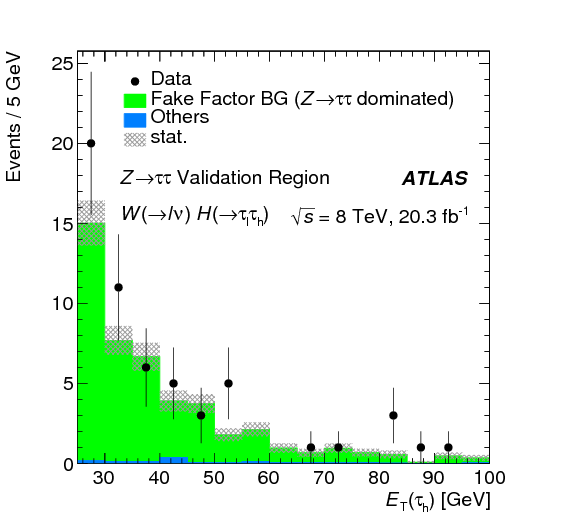
\includegraphics[width=3in]{figures/chapter7/run1_ff_cr.png}
    \caption{Run-1 distribution of the hadronic tau $E_T$ as closure test for the fake factor method in the WH lep-had channel \cite{vh_run1_paper}.}
    \label{fig:run1_ff_cr}
\end{figure}

\subsubsection{WH hadhad Channel}
Initial closure tests for the WH had-had channel using a subset of 2018 data corresponding to a luminosity of roughly 30 fb$^{-1}$ are presented in the following two sections. For these tests, only fake taus are considered and all tau candidates in an event are considered.

\paragraph{Pre-selection}\mbox{} \\
The WH had-had pre-selection region is defined by including all the analysis channel requirements described in Chapter 6 with the exception of the b-jet veto and the lepton-MET $p_T>20$ GeV requirement. Results of the closure test in this region for a variety of kinematics are shown in Figures \ref{fig:presel_taueta} - \ref{fig:presel_met}. Here, tau-1 refers to the highest $p_T$ tau attributed to the Higgs.

These closure tests unfortunately have low statistics (and correspondingly large uncertainties) due to considering only a small subset of the full Run-2 data-set.  Nevertheless, the fake background distributions generally follow the pattern of the data distributions and thus these can be considered a `proof of principle' for the FF software.

\begin{figure}[htb!]
    \centering
    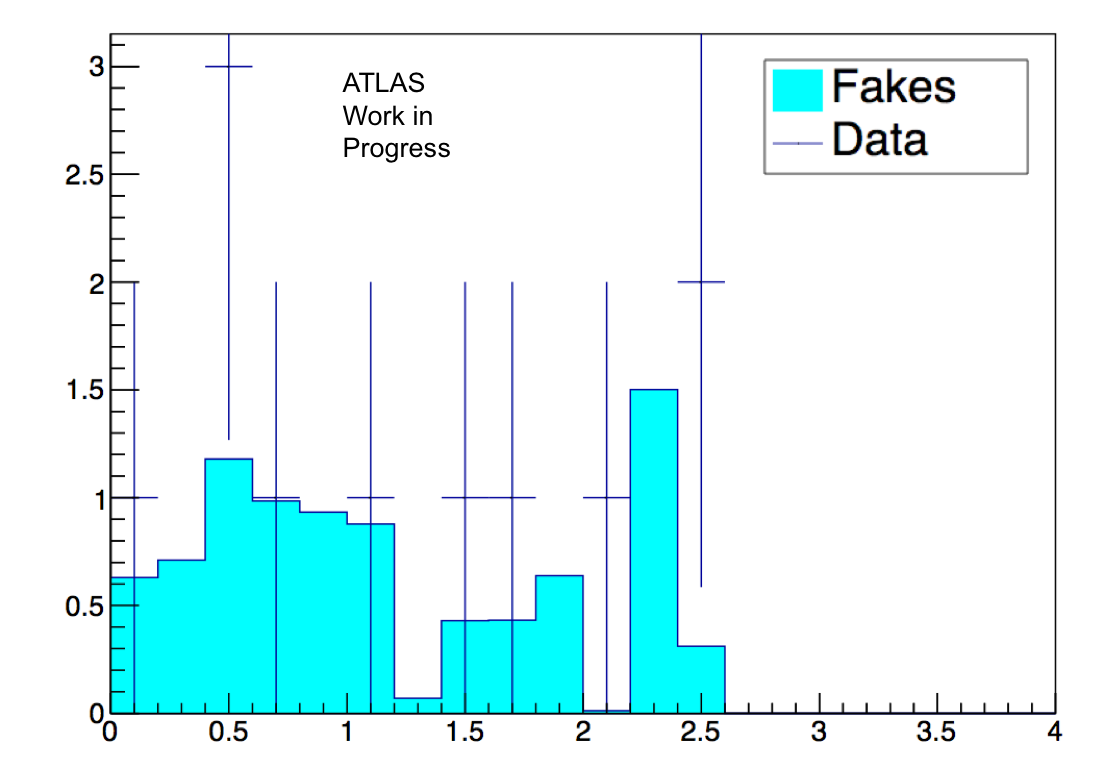
\includegraphics[width=3in]{figures/chapter7/tau1_eta_whpresel.png}
    \caption{WH had-had pre-selection closure test tau-1 $\eta$ distribution.}
    \label{fig:presel_taueta}
\end{figure}

\begin{figure}[htb!]
    \centering
    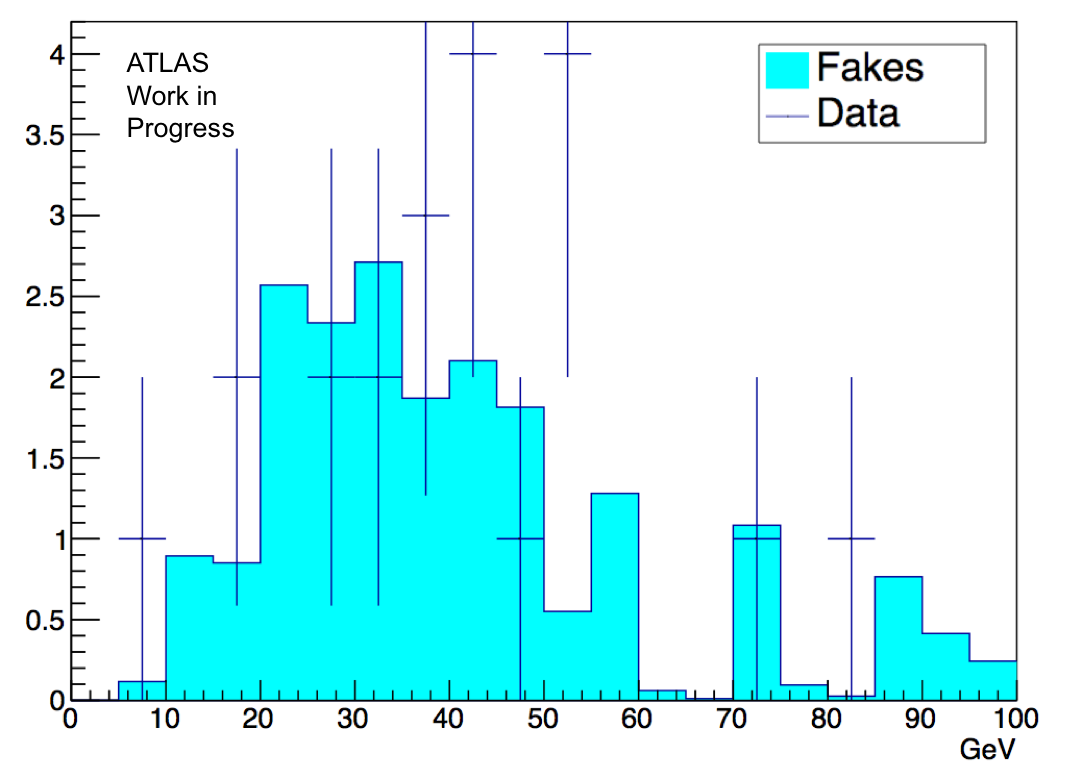
\includegraphics[width=3in]{figures/chapter7/lep_pt_wh_presel.png}
    \caption{WH had-had pre-selection closure test lepton $p_T$ distribution.}
    \label{fig:presel_leppt}
\end{figure}

\pagebreak

\begin{figure}[htb!]
    \centering
    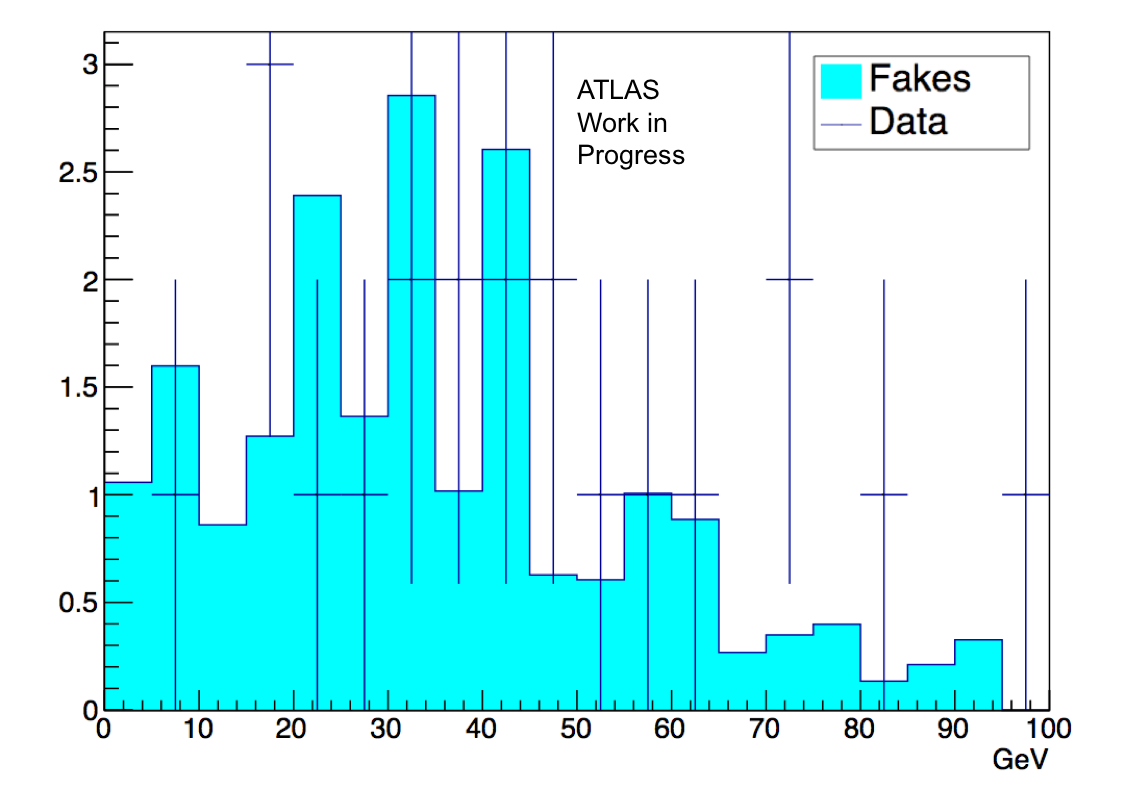
\includegraphics[width=3in]{figures/chapter7/met_whpresel.png}
    \caption{WH had-had pre-selection closure test MET distribution distribution.}
    \label{fig:presel_met}
\end{figure}

\paragraph{$Z\rightarrow\tau\tau$ Control Region}\mbox{} \\

The $Z\rightarrow\tau\tau$ control region for the WH had-had channel is constructed by applying the pre-selection criteria described above with the exception of the oppositely charged tau requirement and with the additional requirements of lep-MET $p_T<$40 GeV and $M_{2T}<60$ GeV. Preliminary results of the closure tests in this region are shown in Figures \ref{fig:leppt_ztautau} and \ref{fig:met_ztautau}. As expected, the distributions exhibit the same low statistics effects seen in the pre-selection region. Additionally, as allowed by the FF equations, some events in the background distribution receive negative weights.

\begin{figure}[htb!]
    \centering
    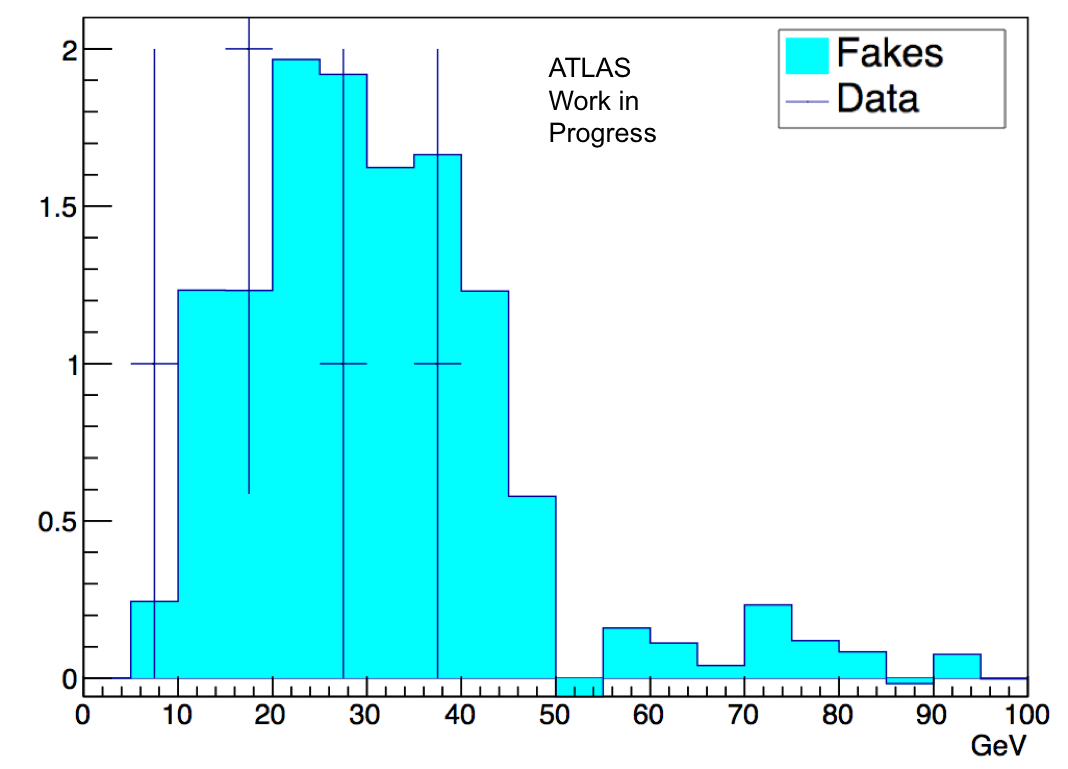
\includegraphics[width=3in]{figures/chapter7/lep_pt_wh_ztautau.png}
    \caption{WH had-had $Z\rightarrow\tau\tau$ closure test lepton $p_T$ distribution.}
    \label{fig:leppt_ztautau}
\end{figure}

\begin{figure}[htb!]
    \centering
    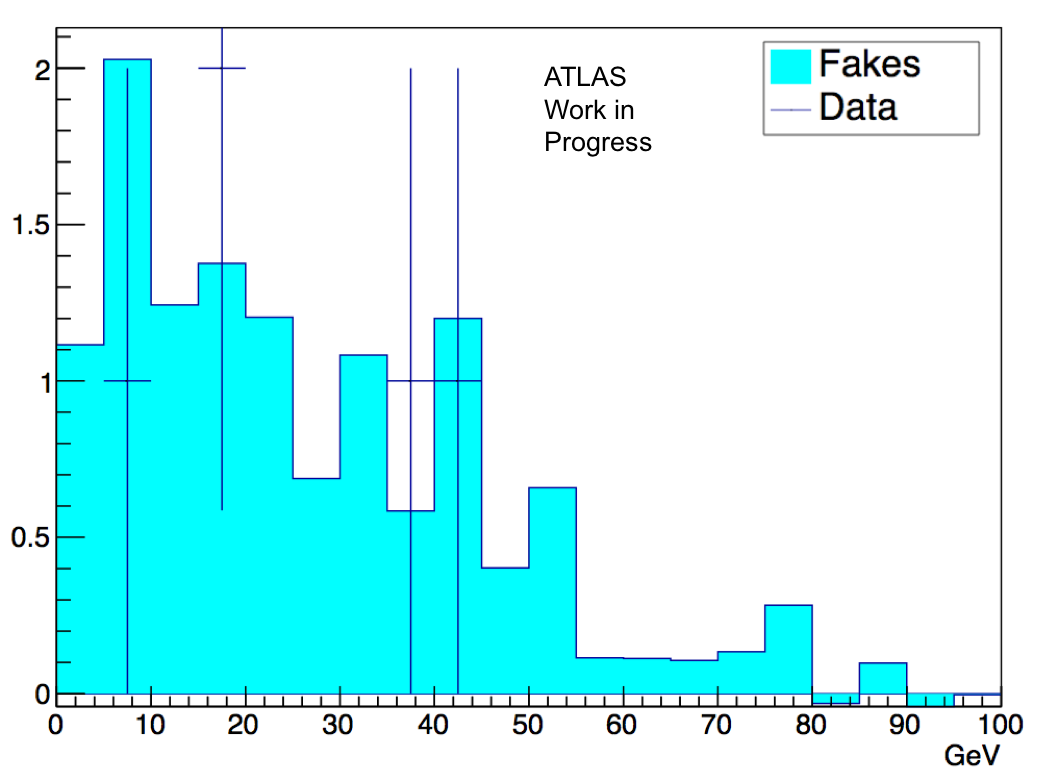
\includegraphics[width=3in]{figures/chapter7/met_wh_ztautau.png}
    \caption{WH had-had $Z\rightarrow\tau\tau$ closure test MET distribution.}
    \label{fig:met_ztautau}
\end{figure}
